\documentclass[10.5pt]{article}
\def\examlang{en}
\def\headyear{2026--2027}
% ===== Preambul comun pentru examen, banca de probleme și setul de exerciții (XeLaTeX) =====
% Statistica piețelor financiare / Statistics of Financial Markets -- Daniel Traian Pele
% Folosire: \documentclass[10.5pt]{article}  \def\examlang{ro} (sau en)  % ===== Preambul comun pentru examen, banca de probleme și setul de exerciții (XeLaTeX) =====
% Statistica piețelor financiare / Statistics of Financial Markets -- Daniel Traian Pele
% Folosire: \documentclass[10.5pt]{article}  \def\examlang{ro} (sau en)  % ===== Preambul comun pentru examen, banca de probleme și setul de exerciții (XeLaTeX) =====
% Statistica piețelor financiare / Statistics of Financial Markets -- Daniel Traian Pele
% Folosire: \documentclass[10.5pt]{article}  \def\examlang{ro} (sau en)  \input{../sfm_exam_preamble}
% Fișierele se compilează din exam/<subfolder>/, deci logo-urile sînt în ../../logos/.
\usepackage{fontspec}
\setmainfont{Helvetica Neue}
\usepackage{amsmath,amssymb}
\usepackage[a4paper,margin=1.9cm,top=2.4cm,headsep=0.5cm,headheight=14pt]{geometry}
\usepackage{graphicx}
\usepackage{float}
\usepackage{booktabs}
\usepackage{array}
\usepackage{enumitem}
\usepackage{xcolor}
\usepackage{fancyhdr}
\usepackage{lastpage}
\usepackage[hidelinks]{hyperref}
\definecolor{spfblue}{RGB}{26,58,110}
\definecolor{spfred}{RGB}{205,0,0}
\graphicspath{{../../logos/}{figs/}{../bank/figs/}{../practice/figs/}}

\providecommand{\examlang}{ro}
\newif\ifen
\def\tmpen{en}\ifx\examlang\tmpen\entrue\else\enfalse\fi

% etichete
\ifen
  \renewcommand{\figurename}{Figure}\renewcommand{\tablename}{Table}
  \newcommand{\coursetitle}{Statistics of Financial Markets}
  \newcommand{\subjword}{Problem}
  \newcommand{\rezword}{Solution.}
  \newcommand{\baremword}{Grading:}
\else
  \renewcommand{\figurename}{Figura}\renewcommand{\tablename}{Tabelul}
  \newcommand{\coursetitle}{Statistica piețelor financiare}
  \newcommand{\subjword}{Subiectul}
  \newcommand{\rezword}{Rezolvare.}
  \newcommand{\baremword}{Barem:}
\fi

% comutator: barem/rezolvare (true) sau subiecte (false)
\newif\ifrez \rezfalse

% antet / subsol
\pagestyle{fancy}
\fancyhf{}
\renewcommand{\headrulewidth}{0.4pt}
\lhead{\small\itshape \coursetitle}
\providecommand{\headyear}{2026}
\rhead{\small\bfseries \headyear}
\cfoot{\small\thepage/\pageref{LastPage}}

\setlength{\parindent}{0pt}
\setlength{\parskip}{0.42ex}
\setlength{\emergencystretch}{3em}

% numerotare automată, continuă, a cerințelor (1, 2, 3, ...)
\newcounter{qq}
\newcommand{\Q}{\refstepcounter{qq}\textbf{\theqq.}~}
% punctaj aliniat la dreapta, pe ultima linie a cerinței
\newcommand{\pts}[1]{\nobreak\hfill\textnormal{\itshape (#1)}\par}

% titlu de subiect: "Subiectul I • Titlu ........ puncte" + linie
\newcommand{\subiect}[3]{%
  \vspace{1.05ex}%
  {\color{spfblue}\bfseries \subjword\ #1 \textbullet\ #2}\hfill{\bfseries #3}\par
  \vspace{0.2ex}{\color{spfblue}\hrule height0.8pt}\vspace{0.7ex}}
% subiect numerotat automat (I, II, ...); argumentul opțional = identificatorul din bancă (vizibil doar în barem)
\newcounter{subj}
\newcommand{\problem}[3][]{%
  \stepcounter{subj}%
  \subiect{\Roman{subj}}{#2\ifrez\if\relax\detokenize{#1}\relax\else\ {\normalfont\footnotesize\color{spfred}[#1]}\fi\fi}{#3}}

% blocul de rezolvare (doar în barem)
\newcommand{\Rez}{\par\vspace{0.2ex}\textit{\rezword}\par\nopagebreak}
\newcommand{\barem}[1]{\par\textit{\baremword\ #1}\par}

% bloc de titlu cu sigle
\newcommand{\titlublock}[1]{%
\begin{center}
  \begin{minipage}[c]{0.16\textwidth}
\includegraphics[height=1.15cm]{ase_logo.png}\end{minipage}%
  \begin{minipage}[c]{0.68\textwidth}\centering
  \ifen
    {\bfseries Bucharest University of Economic Studies}\\[0.2ex]
    Faculty of Cybernetics, Statistics and Economic Informatics\\[0.2ex]
    Course: Statistics of Financial Markets
  \else
    {\bfseries Academia de Studii Economice din București}\\[0.2ex]
    Facultatea de Cibernetică, Statistică și Informatică Economică\\[0.2ex]
    Disciplina: Statistica piețelor financiare
  \fi
  \end{minipage}%
  \begin{minipage}[c]{0.16\textwidth}\raggedleft
\includegraphics[height=0.95cm]{ida_logo.png}\end{minipage}\\[1.2ex]
  {\large\bfseries #1}
\end{center}}

% valori utile generale (z_alpha = cuantila de ordin alpha a distribuției Normale standard)
\newcommand{\valoriutilegen}{%
\ifen Useful values: $z_{0.05}=-1.645$, $z_{0.025}=-1.960$, $z_{0.01}=-2.326$, $\varphi(1.960)=0.0584$,
$\varphi(2.326)=0.0267$, $\ln 2=0.693$, $\sqrt{252}\approx 15.87$, $\sqrt{365}\approx 19.10$,
$\chi^2_{0.95}(1)=3.84$, $\chi^2_{0.95}(2)=5.99$, $\chi^2_{0.95}(10)=18.31$
($z_p$ and $\chi^2_p$ are quantiles of order $p$; $\varphi$ is the standard Normal density).
\else Valori utile: $z_{0,05}=-1{,}645$; $z_{0,025}=-1{,}960$; $z_{0,01}=-2{,}326$; $\varphi(1{,}960)=0{,}0584$;
$\varphi(2{,}326)=0{,}0267$; $\ln 2=0{,}693$; $\sqrt{252}\approx 15{,}87$; $\sqrt{365}\approx 19{,}10$;
$\chi^2_{0,95}(1)=3{,}84$; $\chi^2_{0,95}(2)=5{,}99$; $\chi^2_{0,95}(10)=18{,}31$
($z_p$ și $\chi^2_p$ sînt cuantile de ordin $p$; $\varphi$ este densitatea distribuției Normale standard).\fi}

% titlul capitolului într-un fișier din bancă (folosit doar ca etichetă de build_variant.py)
\newcommand{\banktitle}[2]{}

% Fișierele se compilează din exam/<subfolder>/, deci logo-urile sînt în ../../logos/.
\usepackage{fontspec}
\setmainfont{Helvetica Neue}
\usepackage{amsmath,amssymb}
\usepackage[a4paper,margin=1.9cm,top=2.4cm,headsep=0.5cm,headheight=14pt]{geometry}
\usepackage{graphicx}
\usepackage{float}
\usepackage{booktabs}
\usepackage{array}
\usepackage{enumitem}
\usepackage{xcolor}
\usepackage{fancyhdr}
\usepackage{lastpage}
\usepackage[hidelinks]{hyperref}
\definecolor{spfblue}{RGB}{26,58,110}
\definecolor{spfred}{RGB}{205,0,0}
\graphicspath{{../../logos/}{figs/}{../bank/figs/}{../practice/figs/}}

\providecommand{\examlang}{ro}
\newif\ifen
\def\tmpen{en}\ifx\examlang\tmpen\entrue\else\enfalse\fi

% etichete
\ifen
  \renewcommand{\figurename}{Figure}\renewcommand{\tablename}{Table}
  \newcommand{\coursetitle}{Statistics of Financial Markets}
  \newcommand{\subjword}{Problem}
  \newcommand{\rezword}{Solution.}
  \newcommand{\baremword}{Grading:}
\else
  \renewcommand{\figurename}{Figura}\renewcommand{\tablename}{Tabelul}
  \newcommand{\coursetitle}{Statistica piețelor financiare}
  \newcommand{\subjword}{Subiectul}
  \newcommand{\rezword}{Rezolvare.}
  \newcommand{\baremword}{Barem:}
\fi

% comutator: barem/rezolvare (true) sau subiecte (false)
\newif\ifrez \rezfalse

% antet / subsol
\pagestyle{fancy}
\fancyhf{}
\renewcommand{\headrulewidth}{0.4pt}
\lhead{\small\itshape \coursetitle}
\providecommand{\headyear}{2026}
\rhead{\small\bfseries \headyear}
\cfoot{\small\thepage/\pageref{LastPage}}

\setlength{\parindent}{0pt}
\setlength{\parskip}{0.42ex}
\setlength{\emergencystretch}{3em}

% numerotare automată, continuă, a cerințelor (1, 2, 3, ...)
\newcounter{qq}
\newcommand{\Q}{\refstepcounter{qq}\textbf{\theqq.}~}
% punctaj aliniat la dreapta, pe ultima linie a cerinței
\newcommand{\pts}[1]{\nobreak\hfill\textnormal{\itshape (#1)}\par}

% titlu de subiect: "Subiectul I • Titlu ........ puncte" + linie
\newcommand{\subiect}[3]{%
  \vspace{1.05ex}%
  {\color{spfblue}\bfseries \subjword\ #1 \textbullet\ #2}\hfill{\bfseries #3}\par
  \vspace{0.2ex}{\color{spfblue}\hrule height0.8pt}\vspace{0.7ex}}
% subiect numerotat automat (I, II, ...); argumentul opțional = identificatorul din bancă (vizibil doar în barem)
\newcounter{subj}
\newcommand{\problem}[3][]{%
  \stepcounter{subj}%
  \subiect{\Roman{subj}}{#2\ifrez\if\relax\detokenize{#1}\relax\else\ {\normalfont\footnotesize\color{spfred}[#1]}\fi\fi}{#3}}

% blocul de rezolvare (doar în barem)
\newcommand{\Rez}{\par\vspace{0.2ex}\textit{\rezword}\par\nopagebreak}
\newcommand{\barem}[1]{\par\textit{\baremword\ #1}\par}

% bloc de titlu cu sigle
\newcommand{\titlublock}[1]{%
\begin{center}
  \begin{minipage}[c]{0.16\textwidth}
\includegraphics[height=1.15cm]{ase_logo.png}\end{minipage}%
  \begin{minipage}[c]{0.68\textwidth}\centering
  \ifen
    {\bfseries Bucharest University of Economic Studies}\\[0.2ex]
    Faculty of Cybernetics, Statistics and Economic Informatics\\[0.2ex]
    Course: Statistics of Financial Markets
  \else
    {\bfseries Academia de Studii Economice din București}\\[0.2ex]
    Facultatea de Cibernetică, Statistică și Informatică Economică\\[0.2ex]
    Disciplina: Statistica piețelor financiare
  \fi
  \end{minipage}%
  \begin{minipage}[c]{0.16\textwidth}\raggedleft
\includegraphics[height=0.95cm]{ida_logo.png}\end{minipage}\\[1.2ex]
  {\large\bfseries #1}
\end{center}}

% valori utile generale (z_alpha = cuantila de ordin alpha a distribuției Normale standard)
\newcommand{\valoriutilegen}{%
\ifen Useful values: $z_{0.05}=-1.645$, $z_{0.025}=-1.960$, $z_{0.01}=-2.326$, $\varphi(1.960)=0.0584$,
$\varphi(2.326)=0.0267$, $\ln 2=0.693$, $\sqrt{252}\approx 15.87$, $\sqrt{365}\approx 19.10$,
$\chi^2_{0.95}(1)=3.84$, $\chi^2_{0.95}(2)=5.99$, $\chi^2_{0.95}(10)=18.31$
($z_p$ and $\chi^2_p$ are quantiles of order $p$; $\varphi$ is the standard Normal density).
\else Valori utile: $z_{0,05}=-1{,}645$; $z_{0,025}=-1{,}960$; $z_{0,01}=-2{,}326$; $\varphi(1{,}960)=0{,}0584$;
$\varphi(2{,}326)=0{,}0267$; $\ln 2=0{,}693$; $\sqrt{252}\approx 15{,}87$; $\sqrt{365}\approx 19{,}10$;
$\chi^2_{0,95}(1)=3{,}84$; $\chi^2_{0,95}(2)=5{,}99$; $\chi^2_{0,95}(10)=18{,}31$
($z_p$ și $\chi^2_p$ sînt cuantile de ordin $p$; $\varphi$ este densitatea distribuției Normale standard).\fi}

% titlul capitolului într-un fișier din bancă (folosit doar ca etichetă de build_variant.py)
\newcommand{\banktitle}[2]{}

% Fișierele se compilează din exam/<subfolder>/, deci logo-urile sînt în ../../logos/.
\usepackage{fontspec}
\setmainfont{Helvetica Neue}
\usepackage{amsmath,amssymb}
\usepackage[a4paper,margin=1.9cm,top=2.4cm,headsep=0.5cm,headheight=14pt]{geometry}
\usepackage{graphicx}
\usepackage{float}
\usepackage{booktabs}
\usepackage{array}
\usepackage{enumitem}
\usepackage{xcolor}
\usepackage{fancyhdr}
\usepackage{lastpage}
\usepackage[hidelinks]{hyperref}
\definecolor{spfblue}{RGB}{26,58,110}
\definecolor{spfred}{RGB}{205,0,0}
\graphicspath{{../../logos/}{figs/}{../bank/figs/}{../practice/figs/}}

\providecommand{\examlang}{ro}
\newif\ifen
\def\tmpen{en}\ifx\examlang\tmpen\entrue\else\enfalse\fi

% etichete
\ifen
  \renewcommand{\figurename}{Figure}\renewcommand{\tablename}{Table}
  \newcommand{\coursetitle}{Statistics of Financial Markets}
  \newcommand{\subjword}{Problem}
  \newcommand{\rezword}{Solution.}
  \newcommand{\baremword}{Grading:}
\else
  \renewcommand{\figurename}{Figura}\renewcommand{\tablename}{Tabelul}
  \newcommand{\coursetitle}{Statistica piețelor financiare}
  \newcommand{\subjword}{Subiectul}
  \newcommand{\rezword}{Rezolvare.}
  \newcommand{\baremword}{Barem:}
\fi

% comutator: barem/rezolvare (true) sau subiecte (false)
\newif\ifrez \rezfalse

% antet / subsol
\pagestyle{fancy}
\fancyhf{}
\renewcommand{\headrulewidth}{0.4pt}
\lhead{\small\itshape \coursetitle}
\providecommand{\headyear}{2026}
\rhead{\small\bfseries \headyear}
\cfoot{\small\thepage/\pageref{LastPage}}

\setlength{\parindent}{0pt}
\setlength{\parskip}{0.42ex}
\setlength{\emergencystretch}{3em}

% numerotare automată, continuă, a cerințelor (1, 2, 3, ...)
\newcounter{qq}
\newcommand{\Q}{\refstepcounter{qq}\textbf{\theqq.}~}
% punctaj aliniat la dreapta, pe ultima linie a cerinței
\newcommand{\pts}[1]{\nobreak\hfill\textnormal{\itshape (#1)}\par}

% titlu de subiect: "Subiectul I • Titlu ........ puncte" + linie
\newcommand{\subiect}[3]{%
  \vspace{1.05ex}%
  {\color{spfblue}\bfseries \subjword\ #1 \textbullet\ #2}\hfill{\bfseries #3}\par
  \vspace{0.2ex}{\color{spfblue}\hrule height0.8pt}\vspace{0.7ex}}
% subiect numerotat automat (I, II, ...); argumentul opțional = identificatorul din bancă (vizibil doar în barem)
\newcounter{subj}
\newcommand{\problem}[3][]{%
  \stepcounter{subj}%
  \subiect{\Roman{subj}}{#2\ifrez\if\relax\detokenize{#1}\relax\else\ {\normalfont\footnotesize\color{spfred}[#1]}\fi\fi}{#3}}

% blocul de rezolvare (doar în barem)
\newcommand{\Rez}{\par\vspace{0.2ex}\textit{\rezword}\par\nopagebreak}
\newcommand{\barem}[1]{\par\textit{\baremword\ #1}\par}

% bloc de titlu cu sigle
\newcommand{\titlublock}[1]{%
\begin{center}
  \begin{minipage}[c]{0.16\textwidth}
\includegraphics[height=1.15cm]{ase_logo.png}\end{minipage}%
  \begin{minipage}[c]{0.68\textwidth}\centering
  \ifen
    {\bfseries Bucharest University of Economic Studies}\\[0.2ex]
    Faculty of Cybernetics, Statistics and Economic Informatics\\[0.2ex]
    Course: Statistics of Financial Markets
  \else
    {\bfseries Academia de Studii Economice din București}\\[0.2ex]
    Facultatea de Cibernetică, Statistică și Informatică Economică\\[0.2ex]
    Disciplina: Statistica piețelor financiare
  \fi
  \end{minipage}%
  \begin{minipage}[c]{0.16\textwidth}\raggedleft
\includegraphics[height=0.95cm]{ida_logo.png}\end{minipage}\\[1.2ex]
  {\large\bfseries #1}
\end{center}}

% valori utile generale (z_alpha = cuantila de ordin alpha a distribuției Normale standard)
\newcommand{\valoriutilegen}{%
\ifen Useful values: $z_{0.05}=-1.645$, $z_{0.025}=-1.960$, $z_{0.01}=-2.326$, $\varphi(1.960)=0.0584$,
$\varphi(2.326)=0.0267$, $\ln 2=0.693$, $\sqrt{252}\approx 15.87$, $\sqrt{365}\approx 19.10$,
$\chi^2_{0.95}(1)=3.84$, $\chi^2_{0.95}(2)=5.99$, $\chi^2_{0.95}(10)=18.31$
($z_p$ and $\chi^2_p$ are quantiles of order $p$; $\varphi$ is the standard Normal density).
\else Valori utile: $z_{0,05}=-1{,}645$; $z_{0,025}=-1{,}960$; $z_{0,01}=-2{,}326$; $\varphi(1{,}960)=0{,}0584$;
$\varphi(2{,}326)=0{,}0267$; $\ln 2=0{,}693$; $\sqrt{252}\approx 15{,}87$; $\sqrt{365}\approx 19{,}10$;
$\chi^2_{0,95}(1)=3{,}84$; $\chi^2_{0,95}(2)=5{,}99$; $\chi^2_{0,95}(10)=18{,}31$
($z_p$ și $\chi^2_p$ sînt cuantile de ordin $p$; $\varphi$ este densitatea distribuției Normale standard).\fi}

% titlul capitolului într-un fișier din bancă (folosit doar ca etichetă de build_variant.py)
\newcommand{\banktitle}[2]{}

\renewcommand{\subjword}{Problem}
\newcommand{\pp}[1]{\stepcounter{subj}\subiect{\arabic{subj}}{#1}{}}
\newcommand{\chapterhead}[1]{\par\vspace{1.4ex}{\large\bfseries\color{spfred}#1}\par\vspace{0.4ex}}
\setlist[enumerate]{label=(\alph*),leftmargin=2.2em,itemsep=0.15ex,topsep=0.3ex}
\begin{document}
\titlublock{EXAM PROBLEMS --- PRACTICE SET}

\noindent The problems follow the format of the exam: a short computation followed by the interpretation of the
result. The data are the daily series used in the course (last day: 18 September 2026). Numerical answers are at
the end of the document.
Notation: $R_t$ is the simple return, $r_t=\ln(P_t/P_{t-1})$ the log return, and
$\mathrm{VaR}_\alpha=-q_\alpha$ (VaR 1\% is the loss exceeded on 1\% of days).\par
\vspace{0.4ex}{\small\noindent\valoriutilegen\par}

% ===================================================================================================
\chapterhead{Chapter 1. Data, returns and indicators}

\pp{The return of a portfolio: Banca Transilvania and OMV Petrom in 2025}
The adjusted closing prices were $17.71$ lei (31 December 2024) and $25.52$ lei (31 December 2025) for Banca
Transilvania (TLV), and $0.615$ lei and $0.941$ lei for OMV Petrom (SNP). On 31 December 2024 an investor bought a
portfolio with weights $60\%$ TLV and $40\%$ SNP and held it for the whole year.
\begin{enumerate}
\item Compute the simple return of each stock in 2025.
\item Compute the simple return of the portfolio.
\item Compare the log return of the portfolio with the weighted average of the log returns of the two stocks.
\item Explain why simple returns aggregate across assets, while log returns aggregate over time.
\end{enumerate}

\pp{The drawdown of the BET index in 2020}
Figure~\ref{fig:bet} shows the BET index and its drawdown between 2015 and 2026. The peak before the COVID-19 crash
was $10{,}219.75$ points (23 January 2020), the trough was $7{,}038.95$ points (23 March 2020), and the index
regained its peak level on 13 January 2021.
\begin{figure}[H]\centering
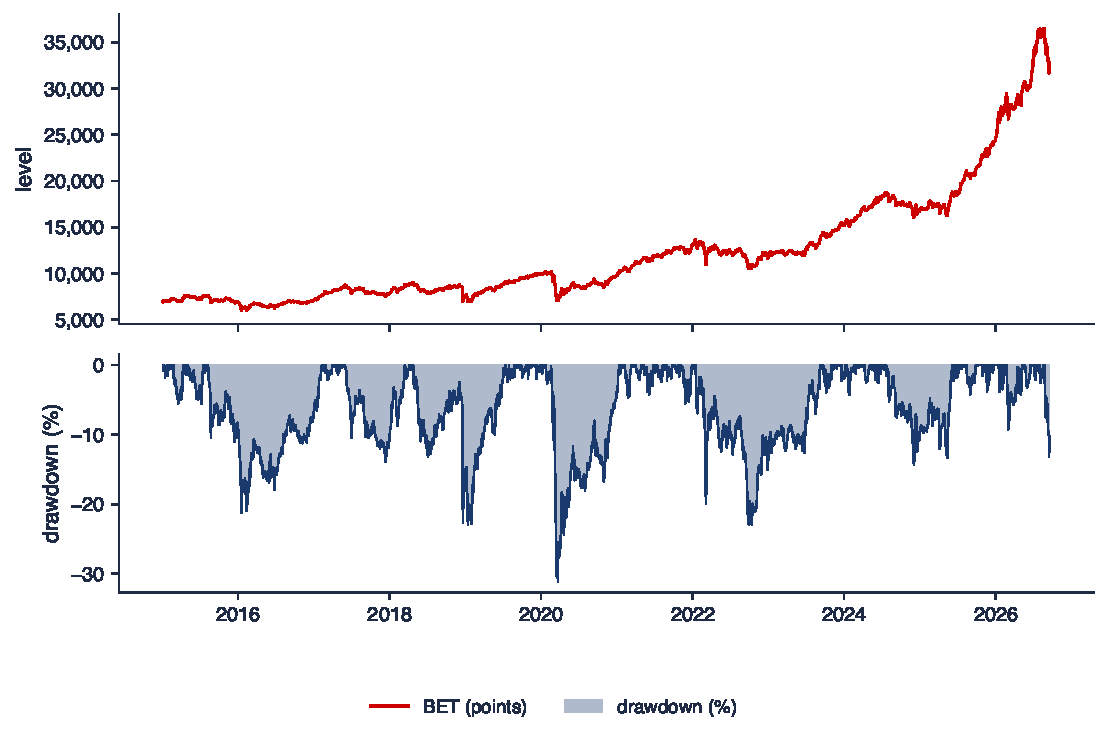
\includegraphics[width=0.66\textwidth]{practice_bet_drawdown_en.pdf}
\caption{The BET index and its drawdown $D_t=P_t/\max_{s\le t}P_s-1$, 2015--2026.}\label{fig:bet}
\end{figure}
\begin{enumerate}
\item Compute the maximum drawdown of the episode.
\item Compute the percentage gain needed to return from the trough to the peak.
\item Interpret the length of the underwater period for an investor with a short horizon.
\end{enumerate}

\pp{The Sharpe ratio and the Sortino ratio: S\&P 500}
For the S\&P 500 (2015--2026, 252 days per year), the annualised mean log return is $11.24\%$, the annualised
volatility is $17.71\%$, and the annualised downside deviation (threshold $\tau=0$) is $\sigma_D=12.82\%$. Take
$r_f=0$.
\begin{enumerate}
\item Compute the Sharpe ratio.
\item Compute the Sortino ratio.
\item Explain why the Sortino ratio is larger than the Sharpe ratio for this series.
\end{enumerate}

% ===================================================================================================
\chapterhead{Chapter 2. Classical distributions and stylised facts}

\pp{The Jarque--Bera test for the DAX}
For the daily log returns of the DAX index (2015--2026), $n=2972$, the skewness is $S=-0.565$ and the excess
kurtosis is $K=9.973$.
\begin{enumerate}
\item Compute the statistic $\mathrm{JB}=\frac{n}{6}\left(S^2+K^2/4\right)$.
\item Compute the contributions of skewness and of kurtosis to the JB statistic.
\item State the decision of the test at the 5\% significance level.
\end{enumerate}

\pp{Aggregational Gaussianity: S\&P 500}
For S\&P 500 log returns (2015--2026), the excess kurtosis is $15.85$ for daily returns ($n=2943$), $10.80$ for
sums over blocks of 5 days ($n=588$) and $4.00$ for sums over blocks of 21 days ($n=140$). Over the 21-day blocks
the skewness is $S=-1.10$.
\begin{enumerate}
\item Test the normality of the 21-day returns with the Jarque--Bera statistic at the 5\% significance level.
\item Explain why the excess kurtosis falls as the horizon grows.
\item Find the degrees of freedom $\nu$ of the Student-$t$ distribution whose excess kurtosis $6/(\nu-4)$ equals
$4.00$.
\end{enumerate}

\pp{The worst day of the BET index}
On 19 December 2018 the BET index fell by $11.89\%$ (log return). Over 2015--2026 ($n=2925$ days) the mean daily
return is $0.053\%$ and the standard deviation is $0.983\%$. Over the same period, 42 days had $|z_t|>3$, where
$z_t=(r_t-\bar r)/s$.
\begin{enumerate}
\item Compute the standardised return of 19 December 2018.
\item Interpret the Normal probability $\Phi(-12.15)\approx 2.8\cdot 10^{-34}$ of such a day.
\item Compare the number of days with $|z_t|>3$ with the number expected under the Normal distribution
($P(|Z|>3)=0.0027$).
\end{enumerate}

% ===================================================================================================
\chapterhead{Chapter 3. $\alpha$-stable distributions}

\pp{Moments and tails of a stable law}
The daily returns of an asset follow an $\alpha$-stable distribution with $\alpha=1.5$. For a large threshold $x$,
$P(X>x)\approx C\,x^{-\alpha}$.
\begin{enumerate}
\item State whether the mean and the variance of the distribution are finite.
\item Compute the ratio $P(X>2x)/P(X>x)$.
\item Compute the ratio $P(X>10x)/P(X>x)$.
\end{enumerate}

\pp{McCulloch's quantile method: BET}
For the daily log returns of the BET index (2015--2026), the empirical quantiles (in \%) are $q_{0.05}=-1.383$,
$q_{0.25}=-0.380$, $q_{0.50}=0.085$, $q_{0.75}=0.543$, $q_{0.95}=1.417$.
\begin{enumerate}
\item Compute $\nu_\alpha=(q_{0.95}-q_{0.05})/(q_{0.75}-q_{0.25})$.
\item Compute $\nu_\beta=(q_{0.95}+q_{0.05}-2q_{0.5})/(q_{0.95}-q_{0.05})$.
\item Interpret the difference between $\nu_\alpha$ and the value $2.44$ of the Normal distribution.
\end{enumerate}

% ===================================================================================================
\chapterhead{Chapter 4. Probability}

\pp{Diversification: BET and S\&P 500}
The standard deviations of daily returns are $0.983\%$ for the BET and $1.116\%$ for the S\&P 500 (2015--2026,
common days), and their correlation is $\rho=0.305$.
\begin{enumerate}
\item Compute the daily standard deviation of the portfolio with weights $50\%$ and $50\%$.
\item Compute the ratio of this standard deviation to the weighted average of the two standard deviations.
\item Compute the annualised volatility of the portfolio (252 days).
\end{enumerate}

\pp{The AR(1) process: S\&P 500}
The first-order autocorrelation of daily S\&P 500 returns (2015--2026) is $-0.13$. Returns are modelled by the AR(1)
process $X_t=\phi X_{t-1}+\varepsilon_t$, with $\phi=-0.13$ and $\mathrm{Var}(\varepsilon_t)=\sigma^2$.
\begin{enumerate}
\item Compute the second-order autocorrelation.
\item Compute the ratio $\mathrm{Var}(X_t)/\sigma^2$.
\item Suggest an explanation for a negative first-order autocorrelation of a stock index.
\end{enumerate}

% ===================================================================================================
\chapterhead{Chapter 5. Heavy tails and extreme value theory}

\pp{A Hill plot for Bitcoin}
Figure~\ref{fig:hill} shows the Hill estimator $\hat\alpha_k$ of the tail index of Bitcoin daily losses
(2015--2026, $n=4278$) as a function of the number $k$ of losses used. For $k=100$, $\hat\alpha=2.69$.
\begin{figure}[H]\centering
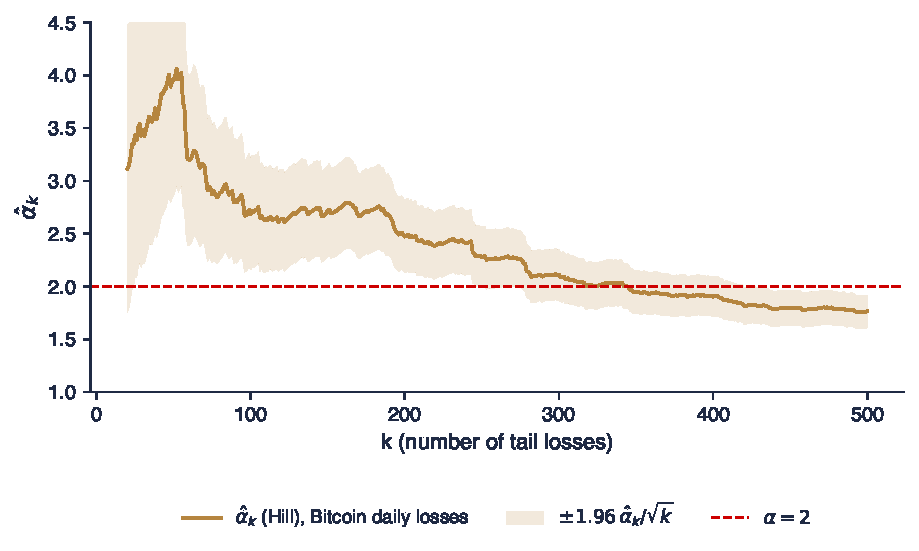
\includegraphics[width=0.62\textwidth]{practice_btc_hill_en.pdf}
\caption{Hill plot: Bitcoin daily losses, 2015--2026.}\label{fig:hill}
\end{figure}
\begin{enumerate}
\item Compute the standard error $\hat\alpha/\sqrt{k}$ and the 95\% confidence interval for $k=100$.
\item State whether, on the basis of this interval, the variance of losses is finite.
\item Explain why the estimates for $k=50$ ($3.96$) and $k=400$ ($1.90$) differ so much.
\end{enumerate}

\pp{A Pareto tail for the S\&P 500}
For the daily losses of the S\&P 500 (2015--2026, in \%), the line fitted on the log--log plot of the tail is
$\ln\hat P(L>x)=-1.391-2.753\ln x$.
\begin{enumerate}
\item Compute the probability of a daily loss larger than 7\%.
\item Express the result of (a) as a mean return period, in years of 252 days.
\item State whether the variance of losses is finite for this tail index.
\end{enumerate}

% ===================================================================================================
\chapterhead{Chapter 6. Model selection and risk management}

\pp{The Normal or the Student-$t$ distribution for Bitcoin?}
On $n=4278$ daily Bitcoin returns (2015--2026), the maximised log-likelihood is $\ell_N=-11{,}415.1$ for the Normal
distribution (2 parameters) and $\ell_t=-10{,}745.8$ for the Student-$t$ distribution with location and scale
(3 parameters, $\hat\nu=2.19$). Use $\ln 4278=8.36$.
\begin{enumerate}
\item Compute the AIC of the two models.
\item Compute the BIC of the two models.
\item State what $\hat\nu=2.19$ implies for the existence of kurtosis.
\end{enumerate}

\pp{The Kupiec test}
A VaR 1\% model records $x=11$ exceptions in $n=500$ days.
\begin{enumerate}
\item Compute the empirical exception rate.
\item Compute $LR_{uc}=-2\ln\dfrac{(1-\alpha)^{n-x}\alpha^x}{(1-\hat\pi)^{n-x}\hat\pi^x}$, with $\hat\pi=x/n$.
\item State the decision at the 5\% significance level.
\end{enumerate}

% ===================================================================================================
\chapterhead{Chapter 7. Efficient markets, random walk and variance-ratio tests}

\pp{Autocorrelations of returns and absolute returns: S\&P 500}
Figure~\ref{fig:acf} shows the autocorrelations of daily S\&P 500 returns and absolute returns (2015--2026,
$n=2943$). The first five autocorrelations of returns are $-0.128$, $0.078$, $-0.031$, $-0.062$, $0.047$.
\begin{figure}[H]\centering
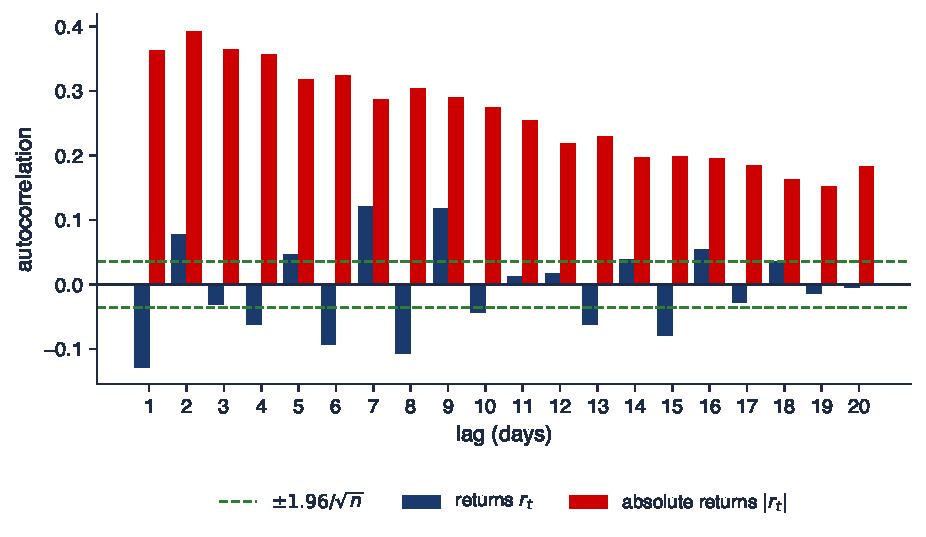
\includegraphics[width=0.62\textwidth]{practice_sp500_acf_en.pdf}
\caption{ACF of $r_t$ and $|r_t|$, S\&P 500, 2015--2026.}\label{fig:acf}
\end{figure}
\begin{enumerate}
\item Compute the limits of the band $\pm 1.96/\sqrt n$.
\item State how many of the first five return autocorrelations lie outside the band.
\item Interpret the difference between the autocorrelations of $r_t$ and those of $|r_t|$.
\end{enumerate}

\pp{The variance ratio from autocorrelations: DAX}
For the DAX (2015--2026, $T=2972$), the first four autocorrelations of daily returns are $-0.020$, $0.034$, $0.014$,
$-0.014$. Under the random walk with constant variance, the standard deviation of $\widehat{\mathrm{VR}}(5)$ is
$0.0402$.
\begin{enumerate}
\item Compute $\mathrm{VR}(5)=1+2\sum_{k=1}^{4}(1-k/5)\hat\rho(k)$.
\item Test the random walk at the 5\% level with $z=(\mathrm{VR}(5)-1)/0.0402$.
\item Interpret the result in terms of weak-form efficiency.
\end{enumerate}

% ===================================================================================================
\chapterhead{Chapter 8. Volatility estimators}

\pp{Range-based estimators: the S\&P 500 on 9 April 2025}
On 9 April 2025 (the day a pause in some tariffs was announced), the S\&P 500 had $O=4965.28$, $H=5481.34$,
$L=4948.43$, $C=5456.90$, and the previous close was $4982.77$. Notation: $u=\ln(H/O)$, $d=\ln(L/O)$,
$c=\ln(C/O)$.
\begin{enumerate}
\item Compute the Parkinson variance $(u-d)^2/(4\ln 2)$ and the corresponding daily volatility.
\item Compute the Garman--Klass variance $0.5(u-d)^2-(2\ln 2-1)c^2$ and the corresponding daily volatility.
\item Explain why Garman--Klass gives a lower value on a day with a strong trend.
\end{enumerate}

\pp{An EWMA update}
Yesterday's EWMA daily volatility was $1.2\%$, and yesterday's return was $-3.5\%$.
\begin{enumerate}
\item Compute today's volatility for $\lambda=0.94$ (RiskMetrics).
\item Compute the half-life of the weights, $\ln 0.5/\ln\lambda$, for $\lambda=0.94$ and for $\lambda=0.97$.
\item State which of the two values of $\lambda$ reacts faster to shocks.
\end{enumerate}

% ===================================================================================================
\chapterhead{Chapter 9. ARCH and GARCH models}

\pp{A GARCH(1,1)-$t$ model for the BET}
The GARCH(1,1) model with Student-$t$ innovations fitted to daily BET returns (in \%, 2015--2026) has
$\hat\omega=0.0691$, $\hat\alpha=0.1846$, $\hat\beta=0.7401$.
\begin{enumerate}
\item Compute the persistence $\alpha+\beta$.
\item Compute the long-run variance and the corresponding annualised volatility (252 days).
\item Compute the half-life of a volatility shock.
\end{enumerate}

\pp{Multi-step volatility forecasts}
With the parameters of the previous problem, the conditional variance for tomorrow is $\sigma^2_{t+1}=4$ (volatility
of 2\%).
\begin{enumerate}
\item Compute the forecast $E_t[\sigma^2_{t+10}]=\bar\sigma^2+(\alpha+\beta)^{9}(\sigma^2_{t+1}-\bar\sigma^2)$.
\item Compute the 10-day volatility as the square root of the sum of the forecasts $E_t[\sigma^2_{t+h}]$,
$h=1,\dots,10$.
\item Compare the result with the rule $\sqrt{10}\,\sigma_{t+1}$.
\end{enumerate}

% ===================================================================================================
\chapterhead{Chapter 10. VaR, ES and backtesting}

\pp{VaR and ES for Banca Transilvania}
For the daily log returns of Banca Transilvania (2015--2026), the mean is $0.106\%$ and the standard deviation is
$1.685\%$. Historical simulation gives VaR 1\% $=4.58\%$ and ES 2.5\% $=4.93\%$.
\begin{enumerate}
\item Compute VaR 1\% and ES 2.5\% under the Normal distribution, with $\mathrm{ES}_\alpha=-\mu+\sigma\varphi(z_\alpha)/\alpha$.
\item Express the historical VaR 1\% in lei for a position of $50{,}000$ lei, using $W(1-e^{-\mathrm{VaR}/100})$.
\item Explain the difference between the results of the two methods.
\end{enumerate}

\pp{Clustered exceptions: the Christoffersen test}
A VaR 1\% model has 10 exceptions in 500 days. Of the 10 exceptions, 3 came right after another exception. The
transition counts are $n_{00}=482$, $n_{01}=7$, $n_{10}=7$, $n_{11}=3$ ($n_{ij}$: days in state $j$ preceded by a
day in state $i$; 1 means an exception).
\begin{enumerate}
\item Compute $\hat\pi_{01}=n_{01}/(n_{00}+n_{01})$.
\item Compute $\hat\pi_{11}=n_{11}/(n_{10}+n_{11})$.
\item State the decision of the independence test, given $LR_{ind}=12.43$.
\end{enumerate}

% ===================================================================================================
\chapterhead{Chapter 11. Fractal markets hypothesis and long memory}

\pp{The Hurst exponent and risk scaling}
The average R/S statistic of a return series is $3.2$ for blocks of $n=10$ days and $42$ for blocks of $n=1000$
days.
\begin{enumerate}
\item Compute the Hurst exponent as the slope in log--log coordinates.
\item Compute the memory parameter $d=H-0.5$ of the corresponding ARFIMA$(0,d,0)$ model.
\item Compute the 20-day VaR 1\% from a daily VaR 1\% of $2.5\%$, with the scaling $h^{H}$ and with the scaling
$\sqrt h$.
\end{enumerate}

% ===================================================================================================
\chapterhead{Chapter 12. Scoring models}

\pp{Altman's Z-score}
A listed manufacturing company has: working capital/total assets $X_1=0.12$; retained earnings/total assets
$X_2=0.25$; EBIT/total assets $X_3=0.08$; market value of equity/total liabilities $X_4=0.60$; sales/total assets
$X_5=1.10$.
\begin{enumerate}
\item Compute $Z=1.2X_1+1.4X_2+3.3X_3+0.6X_4+1.0X_5$.
\item Place the company in Altman's zones ($Z<1.81$ distress zone; $1.81\le Z\le 2.99$ grey zone; $Z>2.99$ safe
zone).
\item State the variable that contributes most to the score.
\end{enumerate}

% ===================================================================================================
\chapterhead{Chapter 13. Machine learning}

\pp{Quantile loss for two VaR forecasts}
Two models forecast the 5\% quantile of the daily return: model A gives $q_A=-2\%$ and model B gives $q_B=-1.5\%$,
on each of 4 days. The realised returns were $1.0\%$, $-0.5\%$, $-2.5\%$, $0.8\%$. The quantile loss is
$\rho_\alpha(u)=u\,(\alpha-\mathbf 1\{u<0\})$, with $u=r_t-q$ and $\alpha=0.05$.
\begin{enumerate}
\item Compute the mean quantile loss of model A.
\item Compute the mean quantile loss of model B.
\item Explain why the quantile loss, and not the squared error, is used to compare VaR forecasts.
\end{enumerate}

% ===================================================================================================
\chapterhead{Chapter 14. Crypto assets}

\pp{Bitcoin at weekends}
For Bitcoin (2015--2026), the standard deviation of daily returns is $2.675\%$ on weekend days and $3.765\%$ on
weekdays. A year has 104 weekend days and 261 weekdays.
\begin{enumerate}
\item Compute the ratio of weekend to weekday volatility.
\item Compute the share of weekend days in the annual variance.
\item Explain why weekends are calmer on the Bitcoin market.
\end{enumerate}

% ===================================================================================================
\chapterhead{Chapter 15. Systemic risk}

\pp{Joint bad days: JPMorgan Chase and the S\&P 500}
Over $n=2932$ common days (2015--2026), a ``bad day'' is a day on which the return is below its own 5\% quantile.
The S\&P 500 had 147 bad days, and on 74 of them JPMorgan Chase also had a bad day.
\begin{enumerate}
\item Compute the number of joint bad days expected if the two series were independent.
\item Compute the conditional probability $P(\text{JPM bad day}\mid\text{S\&P 500 bad day})$.
\item Interpret the result in terms of systemic risk.
\end{enumerate}

% ===================================================================================================
\clearpage
\chapterhead{Answers}
{\small
\begin{enumerate}[label=\textbf{\arabic*.},leftmargin=2.2em,itemsep=0.25ex]
\item (a) TLV $44.10\%$, SNP $52.94\%$. (b) $47.64\%$. (c) $\ln(1.4764)=38.96\%$, against a weighted average of
$38.92\%$: log returns do not aggregate exactly across assets. (d) The simple return of a portfolio is the weighted
average of the simple returns; log returns add up over time.
\item (a) $-31.12\%$. (b) $+45.19\%$. (c) Almost one year below the peak (January 2020 -- January 2021).
\item (a) $0.63$. (b) $0.88$. (c) The downside deviation is smaller than total volatility: part of the variability
comes from rises.
\item (a) $\mathrm{JB}\approx 12{,}475$. (b) Skewness $158$; kurtosis $12{,}317$ (almost all of it).
(c) $\mathrm{JB}\gg 5.99$: normality is rejected.
\item (a) $\mathrm{JB}=121.7>5.99$: normality is rejected at the 21-day horizon too. (b) A sum of several returns
moves towards the Normal distribution (central limit theorem), but slowly, because of volatility clustering.
(c) $\nu=5.5$.
\item (a) $z=-12.15$. (b) Under the Normal distribution such a day would occur about once in $10^{31}$ years: the
Normal model badly understates the tails. (c) Expected $7.9$ days, observed 42: about $5.3$ times more.
\item (a) The mean is finite ($1<\alpha$); the variance is infinite ($2>\alpha$). (b) $2^{-1.5}=0.354$.
(c) $10^{-1.5}=0.032$; for the Normal distribution the ratio is practically zero.
\item (a) $3.03$. (b) $-0.05$. (c) $3.03>2.44$: fatter tails than the Normal distribution ($\alpha<2$);
$\nu_\beta\approx 0$ points to an almost symmetric distribution.
\item (a) $0.848\%$. (b) $0.81$: diversification cuts risk by about 19\%. (c) $0.848\%\cdot\sqrt{252}=13.5\%$.
\item (a) $\phi^2=0.017$. (b) $1/(1-\phi^2)=1.017$. (c) Overreaction to news corrected the next day; for single
stocks, also the bounce of the price between bid and ask.
\item (a) $\mathrm{SE}=0.27$; CI $[2.16,\ 3.22]$. (b) Yes: the interval lies above 2. (c) For small $k$ the
estimator has a large variance; for large $k$ observations from the centre of the distribution enter and bias
appears.
\item (a) $e^{-1.391}\cdot 7^{-2.753}=1.17\cdot 10^{-3}$. (b) About 853 days, i.e.\ $3.4$ years. (c) Yes:
$\alpha=2.753>2$ (moments of order below $\alpha$ are finite).
\item (a) $22{,}834.2$ and $21{,}497.6$. (b) $22{,}846.9$ and $21{,}516.7$; both criteria choose the Student-$t$
distribution. (c) $\nu\le 4$: kurtosis (the fourth moment) is infinite, and the variance exists only just ($\nu>2$).
\item (a) $2.2\%$. (b) $LR_{uc}=5.42$. (c) $5.42>3.84$: correct coverage is rejected (too many exceptions).
\item (a) $\pm 0.036$. (b) Four ($-0.128$, $0.078$, $-0.062$, $0.047$). (c) The sign of returns is hard to predict,
their size is not: the autocorrelations of $|r_t|$ are large and decay slowly (volatility clustering). The band
assumes constant variance, so for $r_t$ it is too narrow.
\item (a) $1.014$. (b) $z=0.36<1.96$: the random walk is not rejected. (c) Five-day DAX returns cannot be predicted
from past returns: the result is consistent with weak-form efficiency.
\item (a) $3.77\cdot 10^{-3}$; $6.14\%$. (b) $1.79\cdot 10^{-3}$; $4.23\%$. (c) The term $-(2\ln 2-1)c^2$ lowers the
variance when the close is near the high.
\item (a) $1.445\%$. (b) $11.2$ days; $22.8$ days. (c) $\lambda=0.94$.
\item (a) $0.925$. (b) $\bar\sigma^2=0.918$; $0.958\%$ per day; $15.2\%$ per year. (c) $8.9$ days.
\item (a) $2.44$ (volatility $1.56\%$). (b) $\sqrt{31.40}=5.60\%$. (c) $\sqrt{10}\cdot 2\%=6.32\%$: the rule
overstates, because volatility reverts to its mean.
\item (a) VaR 1\% $=3.81\%$; ES 2.5\% $=3.83\%$. (b) $2236$ lei. (c) Historical simulation gives values about
$20\%$--$29\%$ higher: the Normal distribution misses the fat tails.
\item (a) $7/489=0.014$. (b) $3/10=0.30$. (c) $12.43>3.84$: independence is rejected; after an exception, a new
exception is about 20 times more likely (the model reacts too slowly to volatility).
\item (a) $H=0.56$. (b) $d=0.06$. (c) $13.3\%$ with $h^H$, against $11.2\%$ with $\sqrt h$.
\item (a) $Z=2.22$. (b) Grey zone. (c) $X_5$ (contribution $1.10$).
\item (a) $(0.150+0.075+0.475+0.140)/4=0.21$. (b) $(0.125+0.050+0.950+0.115)/4=0.31$; model A is better.
(c) The quantile minimises the expected quantile loss (VaR is elicitable for this function); the squared error
targets the mean, not the quantile.
\item (a) $0.71$. (b) $104\cdot 2.675^2/(104\cdot 2.675^2+261\cdot 3.765^2)=16.7\%$, although weekends are $28.5\%$
of days. (c) Traditional markets are closed: there is no macroeconomic news, no institutional flows and no
arbitrage with the ETFs.
\item (a) $2932\cdot 0.05^2=7.3$ days (observed: 74, about 10 times more). (b) $74/147=0.50$, against $0.05$
without conditioning. (c) The bank suffers together with the market: diversification disappears exactly on bad
days, which is what $\Delta$CoVaR and MES measure.
\end{enumerate}}
\end{document}
